\documentclass[a4paper,11pt]{article}

\usepackage[utf8]{inputenc}

\usepackage{graphicx}
\usepackage{caption}
\usepackage{subcaption}

\usepackage{pgfplots}
\pgfplotsset{compat=1.18} 

\usepackage{minted}
\usepackage{siunitx}

\begin{document}

\title{
    \textbf{Linked lists in C}
}
\author{Mo Wang}
\date{Spring 2026}

\maketitle

\section*{Introduction}
This report investigates and delves into performance and behavior of a linked list in C. While linked list offers flexibility by carrying an address of next element of a list, it has some performance bottlenecks in terms of random access and cache locality. The primary goal of this report is to analyze the behavior and key attribute of a linked list and compare these features with arrays.


\section*{Linked list}

A linked list stores a sequence of elements by holding its first element. Each element in a linked list is stored in a cell with an element value and a pointer with the address of the next cell. A null pointer in a linked list cell denotes the last cell in the list, while a null pointer as the first element denotes the absence of elements in the list.

\begin{minted}{c}
typedef struct cell {
    int value;
    struct cell *tail;
} cell;

typedef struct linked {
    cell *first;
} linked;
\end{minted}

The linked list can be created by allocating a memory for the linked list and successively allocating other cells of the list, where one cell address is stored in the previous one's tail. 

A linked list is created by first allocating memory for the list structure itself. Each cell is then successively allocated with each cell's tail pointer storing the address of the next cell in the sequence, hence linking all the cells together. The linked list structure stores a pointer to the first cell as an entry point to the data structure- From a memory perspective, these cells are scattered in dynamic memory, which provides flexibility at the expense of high performance overhead of accessing and searching operations.

\begin{minted}{c}
linked *linked_create() {
    linked *new = (linked*)malloc(sizeof(linked));
    new->first = NULL;
    return new;
}
\end{minted}

\subsection*{Adding an element}

To insert an element at the beginning of a linked list, a new cell is first allocated. The value of the new cell is assigned to the desired element. Its tail pointer is then assigned to point to the current first cell of the list. Finally, the first pointer of the list is updated to point to this new cell, effectively making it the first element of the list. Since the operation requires only one memory allocation and three pointer updates, the time complexity is constant $O(1)$.

\begin{minted}{c}
void linked_add(linked *lnk, int item) {
    cell *new = (cell*) malloc(sizeof(cell));
    new->value = item;
    new->tail = lnk->first;
    lnk->first = new;
}
\end{minted}

\subsection*{Length of linked list}

Because this implemented linked list structure only stores a pointer to first element cell without other necessary metadata, such as the size of the list, calculating the length of the linked list could only be accomplished by traversing the linked list through all the cells. A length counter is held and increments when moving to another cell through the previous cell's tail pointer during traversal. As all cells must be traversed, the complexity of the operation in time is linear to the size of the list $O(n)$.

\begin{minted}{c}
unsigned int linked_length(linked *lnk){
    unsigned int length = 0;
    cell* nxt = lnk->first;
    while (nxt != NULL){
        nxt = nxt->tail;
        length++;
    }
    return length;
}
\end{minted}

\subsection*{Finding an element}

Finding an element requires traversing the linked list from the first element cell to the last one, since the list can only be efficiently accessed sequentially. In this case, the value of each element cell is compared with the search value. The traversal search stops as the element is found. This results in linear time complexity $O(n)$, since each cell has to be traversed in the worst case, while only one cell is traversed in the best case. The operation performs on average $n/2$ traversal in terms of possibility expectation.

\begin{minted}{c}
bool linked_find(linked *lnk, int item){
    cell *nxt = lnk->first;
    while (nxt != NULL && nxt->value != item){
        nxt = nxt->tail;
    }
    return nxt != NULL;
}
\end{minted}

\subsection*{Removing an element}

An element can be removed by finding the element cell by value and therefore unlink it from adjacent cells. The operation is split into two cases: either the first element is targeted for deletion, or the deleted element is in the middle of the list. Removing the first element can be accomplished by updating the first pointer of linked list to the second cell while freeing the first cell. Meanwhile, removing an element in the middle of the array requires finding the element by tracking its previous cell. As the target element cell is found, the previous cell re-links its tail to the element after the target one, while freeing the target afterwards. Although pointer updates and free operations are done in constant time, the target element cell must be located by finding, resulting in linear time complexity $O(n)$, as described earlier.


\begin{minted}{c}
void linked_remove(linked *lnk, int item){
    cell *nxt = lnk->first;
    if (nxt == NULL) return;
    if (nxt->value == item){
        cell *after = nxt->tail;
        free(nxt);
        lnk->first = after;
    }
    else{
        while (nxt->tail != NULL && nxt->tail->value != item){
            nxt = nxt->tail;
        }
        if (nxt->tail != NULL){
            cell *after = nxt->tail->tail;
            free(nxt->tail);
            nxt->tail = after;
        }
    }
}
\end{minted}

\section*{Append operation}
\subsection*{Append Implementation}

When a linked list \texttt{a} of size $n$ is appended to a second linked list \texttt{b} of size $m$, the operation can be performed by updating the tail pointer of the last cell of \texttt{a} so that it points to the first cell of \texttt{b}. Afterwards, the second linked list clears its own cells by setting its head pointer to \texttt{null}. Because the linked list structure does not maintain a direct pointer to the last element, locating the final cell of \texttt{a} requires a full traversal of its $n$ elements, resulting in a linear-time search.

As a result, the overall time complexity of appending one linked list to another in this scenario is $O(n)$, where $n$ is the number of elements in the first linked list. This contrasts with an implementation that maintains a direct tail pointer for each linked list, which would allow appending in $O(1)$ constant time, since the last element could be accessed immediately without traversal.

\begin{minted}{c}
void linked_append(linked *a, linked *b) {
    cell *nxt = a->first;
    cell *prv = NULL;
    while(nxt != NULL) {
        prv = nxt;
        nxt = nxt->tail;
    }
    if (prv == NULL){
        a->first = b->first;
    }
    else{
        prv->tail = b->first;
    }
    b->first = NULL;
}
\end{minted}

\subsection*{Benchmark result: Variable-Fixed Append}
The benchmark results conform the linear growth in running time for the append operation when the first linked list increases in size, consistent with the theoretical time complexity. As shown in Figure~1, the running time exhibits the expected $O(n)$ behavior when the fist linked list varies in length while the second linked list remains fixed at 8192 elements. The corresponding execution times are provided in Table~1.

\begin{table}[h]
\begin{center}
\begin{tabular}{l|ccccccc}
\textbf{Size}
    & 1024 & 2048 & 4196 & 8192 & 16384 & 32768 & 65535 \\
\hline
\textbf{Time (ns)}
    & $3.7\times10^{3}$
    & $6.6\times10^{3}$
    & $1.2\times10^{4}$
    & $2.4\times10^{4}$
    & $4.7\times10^{4}$
    & $9.4\times10^{4}$
    & $1.9\times10^{5}$ \\
\end{tabular}
\caption{Minimum time per loop for append benchmark (transposed)}
\label{tab:append-min-times}
\end{center}
\end{table}

\begin{figure}[h]
  \centering
  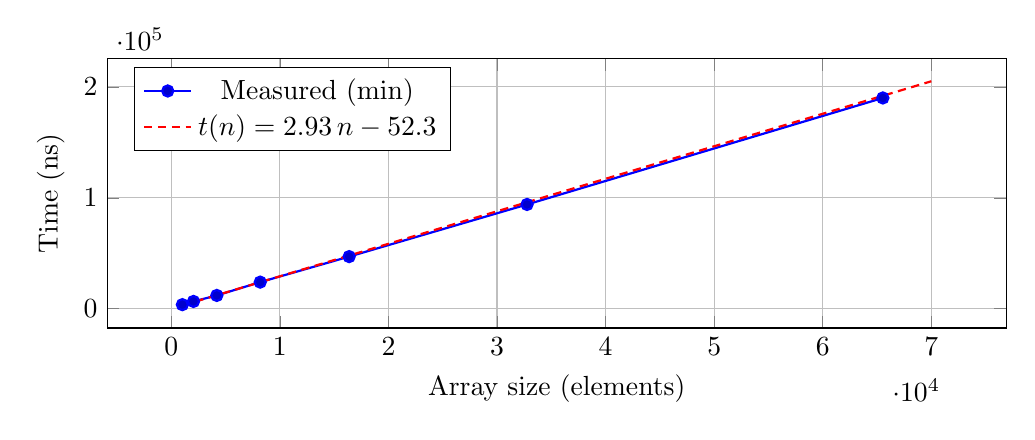
\begin{tikzpicture}
    \begin{axis}[
      xlabel={Array size (elements)},
      ylabel={Time (ns)},
      width=13cm, height=5cm,
      grid=major,
      legend pos=north west,
      ymajorgrids=true,
      xmajorgrids=true
    ]

      % ----------------------------------------------------------
      % Measured MIN times
      % ----------------------------------------------------------
      \addplot+[
        mark=*,
        thick,
        color=blue
      ] coordinates {
        (1024,   3.7e3)
        (2048,   6.6e3)
        (4196,   1.2e4)
        (8192,   2.4e4)
        (16384,  4.7e4)
        (32768,  9.4e4)
        (65535,  1.9e5)
      };
      \addlegendentry{Measured (min)}

      % ----------------------------------------------------------
      % Linear regression fit: t(n) = 2.93 n - 52.3
      % ----------------------------------------------------------
      \addplot[
        red,
        thick,
        densely dashed,
        domain=1000:70000,
        samples=40
      ] {2.93 * x - 52.3};
      \addlegendentry{$t(n)=2.93\,n - 52.3$}

    \end{axis}
  \end{tikzpicture}
  \caption{Minimum measured time per loop with fitted linear regression}
  \label{fig:append-min-times-fitted}
\end{figure}

\subsection*{Benchmark result: Fixed-Variable Append}
Switching the roles of the two linked lists—keeping the first list at a fixed size while allowing the second to grow—results in a constant-time growth pattern, as shown in Figure~2, with the corresponding execution times listed in Table~2. This observation is consistent with the theoretical performance analysis: only the last cell of the fixed linked list must be traversed before the constant-time pointer update can be applied. Consequently, the running time remains bounded by a constant and exhibits an overall time complexity of $O(1)$ for this configuration.

\begin{table}[h]
\begin{center}
\begin{tabular}{l|ccccccc}
\textbf{Size}
    & 1024 & 2048 & 4196 & 8192 & 16384 & 32768 & 65535 \\
\hline
\textbf{Time (ns)}
    & $2.4\times10^{4}$
    & $2.4\times10^{4}$
    & $2.4\times10^{4}$
    & $2.4\times10^{4}$
    & $2.4\times10^{4}$
    & $2.4\times10^{4}$
    & $2.4\times10^{4}$ \\
\end{tabular}
\caption{Minimum time per loop (transposed)}
\label{tab:min-benchmark}
\end{center}
\end{table}

\begin{figure}[h]
  \centering
  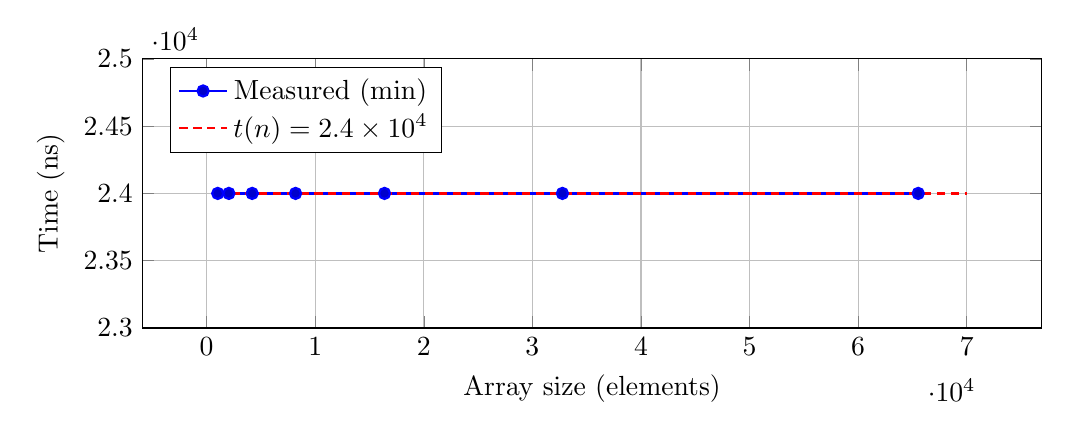
\begin{tikzpicture}
    \begin{axis}[
      xlabel={Array size (elements)},
      ylabel={Time (ns)},
      width=13cm, height=5cm,
      grid=major,
      legend pos=north west,
      ymajorgrids=true,
      xmajorgrids=true,
      ymin=23000,
      ymax=25000
    ]

      % ----------------------------------------------------------
      % Measured MIN times
      % ----------------------------------------------------------
      \addplot+[
        mark=*,
        thick,
        color=blue
      ] coordinates {
        (1024,   2.4e4)
        (2048,   2.4e4)
        (4196,   2.4e4)
        (8192,   2.4e4)
        (16384,  2.4e4)
        (32768,  2.4e4)
        (65535,  2.4e4)
      };
      \addlegendentry{Measured (min)}

      % ----------------------------------------------------------
      % Constant fitted line t(n) = 2.4e4
      % ----------------------------------------------------------
      \addplot[
        red,
        thick,
        densely dashed,
        domain=1000:70000,
        samples=2
      ] {2.4e4};
      \addlegendentry{$t(n)=2.4\times10^{4}$}

    \end{axis}
  \end{tikzpicture}
  \caption{Minimum measured time per loop with fitted constant regression}
  \label{fig:min-times-constant-fit}
\end{figure}

\section*{Comparison with an array}

If the append operation were implemented using arrays instead of linked lists, the procedure would require allocating a new array large enough to hold both inputs, copying all $n$ elements of the first array into the new space, and then copying the $m$ elements of the second array after them. Because arrays have fixed size, this full copy must be performed whenever two arrays are appended.

The cost of appending two arrays is therefore dominated by copying all $n + m$ elements, giving a time complexity of $O(n+m)$. In contrast, the linked-list append only needs to traverse the first list before updating a single pointer, which results in $O(n)$ time without a tail pointer and can be reduced to $O(1)$ if a tail pointer is maintained. In Figure~3, this linear copying cost is reflected in the benchmark results, with execution time data shown in Table~3.

\begin{table}[h]
\begin{center}
\begin{tabular}{l|ccccccc}
\textbf{Size}
    & 1024 & 2048 & 4196 & 8192 & 16384 & 32768 & 65535 \\
\hline
\textbf{Time (ns)}
    & $2.0\times10^{4}$
    & $2.2\times10^{4}$
    & $2.7\times10^{4}$
    & $4.5\times10^{4}$
    & $6.2\times10^{4}$
    & $8.3\times10^{4}$
    & $1.5\times10^{5}$ \\
\end{tabular}
\caption{Minimum time per loop vs. input size (transposed)}
\label{tab:min-times-latest}
\end{center}
\end{table}

\begin{figure}[h]
  \centering
  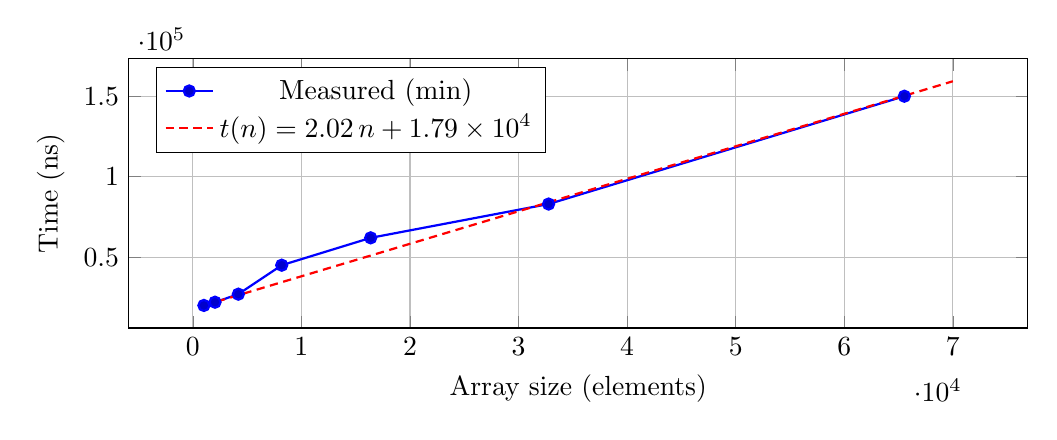
\begin{tikzpicture}
    \begin{axis}[
      xlabel={Array size (elements)},
      ylabel={Time (ns)},
      width=13cm, height=5cm,
      grid=major,
      legend pos=north west,
      ymajorgrids=true,
      xmajorgrids=true
    ]

      % ---------------------------
      % Measured MIN times
      % ---------------------------
      \addplot+[
        mark=*,
        thick,
        color=blue
      ] coordinates {
        (1024,   2.0e4)
        (2048,   2.2e4)
        (4196,   2.7e4)
        (8192,   4.5e4)
        (16384,  6.2e4)
        (32768,  8.3e4)
        (65535,  1.5e5)
      };
      \addlegendentry{Measured (min)}

      % ---------------------------
      % Linear fit: t(n) ≈ 2.02 n + 1.79e4
      % Keep domain small to avoid timeouts
      % ---------------------------
      \addplot[
        red,
        thick,
        densely dashed,
        domain=1000:70000,
        samples=40
      ] {2.02 * x + 1.79e4};
      \addlegendentry{$t(n)=2.02\,n + 1.79\times10^{4}$}

    \end{axis}
  \end{tikzpicture}
  \caption{Minimum time per loop with fitted linear trend}
  \label{fig:min-times-latest}
\end{figure}

\section*{Stack implementation using a linked list}

A stack follows the Last-In–First-Out (LIFO) principle and can be implemented naturally using a linked list. A \texttt{push} operation inserts a new element at the head of the list, while a \texttt{pop} operation removes and returns the head element. Since both operations modify only the first node, they run in constant time $O(1)$.

\begin{minted}{c}
void linked_stack_push(linked_stack *lnk, int item) {
    linked_stack_cell *new_cell = malloc(sizeof(linked_stack_cell));
    new_cell->value = item;
    new_cell->tail = lnk->first;
    lnk->first = new_cell;
}

int linked_stack_pop(linked_stack *lnk) {
    if (lnk->first == NULL) return 0;
    linked_stack_cell *first_cell = lnk->first;
    int value = first_cell->value;
    lnk->first = first_cell->tail;
    free(first_cell);
    return value;
}
\end{minted}

A linked-list-based stack grows dynamically with no need for resizing and supports $O(1)$ insertion and removal at the head. However, each push requires a heap allocation, and each pop requires a deallocation. This leads to pointer chasing, poor cache locality, and higher constant factors compared to arrays.

An array-based stack also offers amortized $O(1)$ push and $O(1)$ pop. Resizing the array is occasionally required when the capacity is exceeded, but the amortized cost remains constant. In practice, array stacks are typically faster because the data is stored in contiguous memory, providing excellent cache performance and minimal overhead per operation.

In summary, both implementations offer the same asymptotic performance, but the array stack is generally faster in real-world execution, while the linked-list stack provides simpler dynamic growth and removes the need for manual capacity management.

\section*{Conclusion}

Linked lists provide flexible dynamic structures, while arrays benefit from contiguous memory and strong cache locality. In a linked list, searching is $O(n)$, whereas insertion or deletion at a known position is $O(1)$.

The first benchmark varied the size of list $a$ while appending it to a fixed-size list $b$. Without a tail pointer, the append operation must traverse all $n$ nodes of $a$, giving the expected linear time $O(n)$. In the second benchmark, list $a$ remained fixed while list $b$ grew. Because the algorithm only traverses the fixed list, the running time stays constant and exhibits $O(1)$ behavior.

For arrays, appending two sequences of size $n$ and $m$ requires allocating a new array and copying all elements, resulting in $O(n+m)$ time. Linked lists avoid this full copy and only traverse the destination list; with a tail pointer the operation can be reduced to $O(1)$, see Table~\ref{tab:linkedlist-vs-array}.

\begin{table}[h]
\centering
\begin{tabular}{l|p{5cm}|p{5cm}}
\textbf{Aspect} & \textbf{Linked list} & \textbf{Array} \\ \hline
Variable--fixed append & $O(n)$ traversal & $O(n+m)$ copy \\ \hline
Fixed--variable append & $O(1)$ & $O(n+m)$ copy \\ \hline
Memory behavior & Non-contiguous & Contiguous \\ \hline
Practical performance & Flexible but slower & Typically faster \\ \hline
\end{tabular}
\caption{Comparison of linked lists and arrays}
\label{tab:linkedlist-vs-array}
\end{table}

Table~\ref{tab:stack-comparison} summarizes the stack implementations. Both stacks support $O(1)$ push and pop in theory, 
but differ in practice: linked lists require heap allocation per push and pointer chasing on pop, while arrays operate in 
contiguous memory and only occasionally resize.

\begin{table}[h]
\centering
\begin{tabular}{l|p{5cm}|p{5cm}}
\textbf{Aspect} & \textbf{Linked-list stack} & \textbf{Array stack} \\ \hline
Push / Pop cost & $O(1)$ & Amortized $O(1)$ \\ \hline
Memory allocation & Allocate/free per op & Rare resizing \\ \hline
Cache locality & Poor & Excellent \\ \hline
Overhead & Pointer + allocation cost & Minimal \\ \hline
Typical performance & Slower & Faster \\ \hline
\end{tabular}
\caption{Stack implementations}
\label{tab:stack-comparison}
\end{table}

Overall, linked lists offer flexible growth and simple structural modifications, while arrays provide better real-world performance due to contiguous storage and efficient memory access.

\end{document}